\section{H-Bridge}

%----------------------------------------------------------------------------------------
%	H-BRIDGE SUBESCTION
%----------------------------------------------------------------------------------------
\subsection{Definition}
An H bridge is an electronic circuit that enables a voltage to be applied across a load in either direction. These circuits are often used in robotics and other applications to allow DC motors to run forwards or backwards.
Most DC-to-AC converters (power inverters), most AC/AC converters, the DC-to-DC push–pull converter, most motor controllers, and many other kinds of power electronics use H bridges. In particular, a bipolar stepper motor is almost invariably driven by a motor controller containing two H bridges.\\

\centerline{
	\centering
	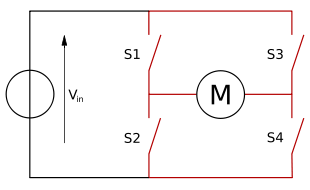
\includegraphics[width=1.0\textwidth]{overview/images/H_bridge.png}
}

%----------------------------------------------------------------------------------------
%	OPERATION SUBESCTION
%----------------------------------------------------------------------------------------
\newpage
\subsection{Operation}
The H-bridge arrangement is generally used to reverse the polarity/direction of the motor, but can also be used to 'brake' the motor, where the motor comes to a sudden stop, as the motor's terminals are shorted, or to let the motor 'free run' to a stop, as the motor is effectively disconnected from the circuit. The following table summarises operation, with S1-S4 corresponding to the diagram above.
\\\\
\centerline{
	\centering
	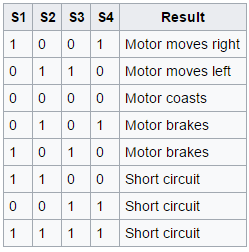
\includegraphics[width=1.0\textwidth]{overview/images/operations.png}
}